%!TEX root=paper/paper.tex
\subsection{Learning the classifier}\label{sec:clf_classifier}

\PM{Logistic regression and NN}
We have so far assumed that $g$ can combine an arbitrary subset of features and provide a distribution $P(Y = y)$---for example, a Gaussian Naive Bayes (NB) model trained on the fully-observed data.
However, a Naive Bayes classifier suffers from its restrictive independence assumptions.
Since discriminative classifiers commonly provide better performance, we'd like to use a \textbf{logistic regression} classifier.
Nearest Neighbor methods also provide a robust classifier for partially observed data, but are slow for large datasets.
We consider them in this exposition, but do not use them in final policy learning experiments due to this problem.

\PM{Missing features}
This presents a new challenge: at test time, some feature values are missing.
If the classifier is trained exclusively on fully-observed data, then the feature value statistics at test time will not match, resulting in poor performance.
Therefore, we need to learn classifier weights on a distribution of data that exhibits the pattern of missing features induces by the policy $\pi$.

\begin{algorithm}[]
\SetKwFunction{ComputeRewards}{ComputeRewards}
\SetKwFunction{GatherSamples}{GatherSamples}
\SetKwFunction{UpdatePolicy}{UpdatePolicy}
\SetKwFunction{UpdateClassifier}{UpdateClassifier}

\SetAlgoLined
\KwIn{$\mathcal{D} = \{x_n, y_n\}_{n=1}^N$; $\mathcal{L}_\mathcal{B}$}
\KwResult{Trained $\pi$, $g$}
\BlankLine
$\pi_0 \leftarrow$ random\;
\For {$i \leftarrow 1$ \KwTo max\_iterations} {
    States, Actions, Costs, Labels $\leftarrow$ \GatherSamples{$\mathcal{D}$, $\pi_{i-1}$}\;
    $g_i \leftarrow$ \UpdateClassifier{States, Labels}\;
    Rewards $\leftarrow$ \ComputeRewards{States, Costs, Labels, $g_i, \mathcal{L}_\mathcal{B}, \gamma$}\;
    $\pi_i \leftarrow$ \UpdatePolicy{States, Actions, Rewards}\;
}
\caption{Because reward computation depends on the classifier, and the distribution of states depends on the policy, $g$ and $\pi$ are trained iteratively.\label{alg:learning}}
\end{algorithm}


\PM{Joint learning}
At the same time, learning the policy depends on the classifier $g$, used in the computation of the rewards.
For this reason, the policy and classifier need to be learned jointly: \autoref{alg:learning} gives the iterative procedure.
In summary, we start from random $\pi$ and $g$, gather a batch of trajectories.
The batch is used to update both $g$ and $\pi$.
Then new trajectories are generated with the updated $\pi$, rewards are computed using the updated $g$, and the process is repeated.
This is a variant of generalized policy iteration \cite{Sutton1998}.

\subsubsection{Unobserved value imputation}

\PM{Formulation}
Unlike the Naive Bayes classifier, the logistic regression classifier is not able to use an arbitrary subset of features $\mathcal{H}_\pi$, but instead operates on feature vectors of a fixed size.
To represent the feature vector of a fully observed instance, we write $\mathbf{x} = [h_1(x), \dots, h_f(x)]$.
In case that $\mathcal{H}_\pi \subset \mathcal{H}$, we need to fill in unobserved feature values in the vector.

\PM{Formulation}
We can think of the policy as a test-time feature selection function $o(x, b): \mathcal{X} \times \mathbb{R} \mapsto \mathbb{B}^F$, where $\mathbb{B} \in \{0, 1\}$, and $b \in [0, 1]$ is given and specifies the fractional selection \emph{budget}.
Applied to $x$, $o(x, b)$ gives the binary selection vector $\mathbf{o}$ which splits $\mathbf{x}$ it into observed and unobserved parts such that $\mathbf{x}^m = [\mathbf{x}^\text{o}, \mathbf{x}^\text{u}]$.
$X^c$ denotes the fully observed $N \times F$ training set.
We assume that we have only sequential access to the missing-feature test instances $\mathbf{x}^m$.

\paragraph{Mean imputation}

A basic strategy is \textbf{mean imputation}: filling in with the mean value of the feature.
We simply replace the missing value in $X^m$ with their row mean in $X^c$.
Because our data is always zero-mean, this amounts to simply replacing the value with $0$.
\begin{align}
\mathbf{x}_\pi = \left[ h_i(x) : \left\{ \begin{array}{rl}
 h_i(x) &\mbox{ if $h_i \in \mathcal{H}_{\pi(x)}$} \\
 \bar{\mathbf{h}}_i &\mbox{ otherwise}
\end{array} \right. \right]
\end{align}

\paragraph{Joint Gaussian model}

\PM{Gaussian Imputation}
If we assume that $\mathbf{x}$ is distributed according to a multivariate Gaussian $\mathbf{x} \sim \mathcal{N}(\mathbf{0}, \Sigma)$, where $\Sigma$ is the sample covariance $X^T X$ and the data is standardized to have zero mean, then it is possible to do \textbf{Gaussian imputation}.
Given a feature subset $\mathcal{H}_\pi$, we write:
\begin{equation}
\mathbf{x}_\pi = \begin{bmatrix} \mathbf{x}^\text{o}\\  \mathbf{x}^\text{u} \end{bmatrix} \sim \mathcal{N} \left( \mathbf{0}, \begin{bmatrix} \mathbf{A} & \mathbf{C}\\ \mathbf{C}^T & \mathbf{B} \end{bmatrix} \right)
\end{equation}
where $\mathbf{x}^\text{o}$ and $\mathbf{x}^\text{u}$ represent the respectively observed and unobserved parts of the full feature vector $\mathbf{x}$, $\mathbf{A}$ is the covariance matrix of $\mathbf{x}^\text{o}$, $\mathbf{B}$ is the covariance matrix of $\mathbf{x}^\text{u}$, and $C$ is the cross-variance matrix that has as many rows as the size of $\mathbf{x}^\text{o}$ and as many columns as the size of $\mathbf{x}^\text{u}$ \parencite{Roweis-gaussian-identities}.
In this case, the distribution over unobserved variables conditioned on the observed variables is given as
$\mathbf{x}^\text{u} \mid \mathbf{x}^\text{o} \sim \mathcal{N} \left( \mathbf{C}^T \mathbf{A}^{-1} \mathbf{x}^\text{o},\, \mathbf{B} - \mathbf{C}^T \mathbf{A}^{-1} \mathbf{C} \right)$.

We can make a modeling assumption that allows another imputation method.
Specifically, we assume that $\mathbf{x}$ is distributed according to a multivariate Gaussian $\mathbf{x} \sim \mathcal{N}(\mathbf{0}, \Sigma)$, where $\Sigma$ is the sample covariance $X^T X$ and the data is standardized to have zero mean.

For a test instance with missing features, we can write
\begin{equation}
\mathbf{x} = \begin{bmatrix} \mathbf{x}^\text{o}\\  \mathbf{x}^\text{u} \end{bmatrix} \sim \mathcal{N} \left( \mathbf{0}, \begin{bmatrix} \mathbf{A} & \mathbf{C}\\ \mathbf{C}^T & \mathbf{B} \end{bmatrix} \right)
\end{equation}
where $\mathbf{A}$ is the covariance matrix of $\mathbf{x}^\text{o}$, $\mathbf{B}$ is the covariance matrix of $\mathbf{x}^\text{u}$, and $C$ is the cross-variance matrix that has as many rows as the size of $\mathbf{x}^\text{o}$ and as many columns as the size of $\mathbf{x}^\text{u}$ \cite{Roweis-gaussian-identities}.

In this case, the distribution over unobserved variables conditioned on the observed variables is given by
\begin{equation}
\mathbf{x}^\text{u} \mid \mathbf{x}^\text{o} \sim \mathcal{N} \left( \mathbf{C}^T \mathbf{A}^{-1} \mathbf{x}^\text{o},\, \mathbf{B} - \mathbf{C}^T \mathbf{A}^{-1} \mathbf{C} \right)
\end{equation}

\PM{Complexity}
After computing the complete covariance matrix $\Sigma$, which takes $O(N^3)$ time, we need to make $N'$ test-time predictions.
In the course of the predictions, we may need to compute at most $\min(N', 2^F)$ unique matrix inversions (again in $O(N^3)$).
The size of the matrices being inverted is proportional to the budget $b$, making this method slower for larger budgets.

\paragraph{k-NN Imputation and Prediction}
In the Gaussian method, we want to use some knowledge of the feature covariance to fill in the missing values.
Instead of learning anything, we could go directly to the source of the covariances---the actual feature values for all points in the training set.
The family of Nearest Neighbor methods takes this approach.
The algorithm for imputation is simple: find the nearest neighbors in the observed dimensions, and use their averaged values to fill in the unobserved dimensions.

For $\mathbf{X}^m$, we find the $k$ nearest neighbors with the highest dot product similarity $\mathbf{x}^{cT} \mathbf{x^m}$ or lowest Euclidean distance $\| \mathbf{x}^{c} - \mathbf{x}^{m} \|$, using only the features that are observed in $\mathbf{x}^{m}$.
For \textbf{imputation}, the unobserved values are set to the average across these nearest neighbors for that dimension.
Similarly, we do \textbf{classification} by returning the mode label of the nearest neighbors.

\PM{Complexity}
Finding the nearest neighbors by dot product similarity is $O(NF'^2)$, and Euclidean distance is the same with an additional constant term.
$F'S$ is the number of observed dimensions, which grows proportionally with budget $b$, making this method more expensive with increased budget.

\subsubsection{Learning more than one classifier}

\begin{figure}[ht]
\centering
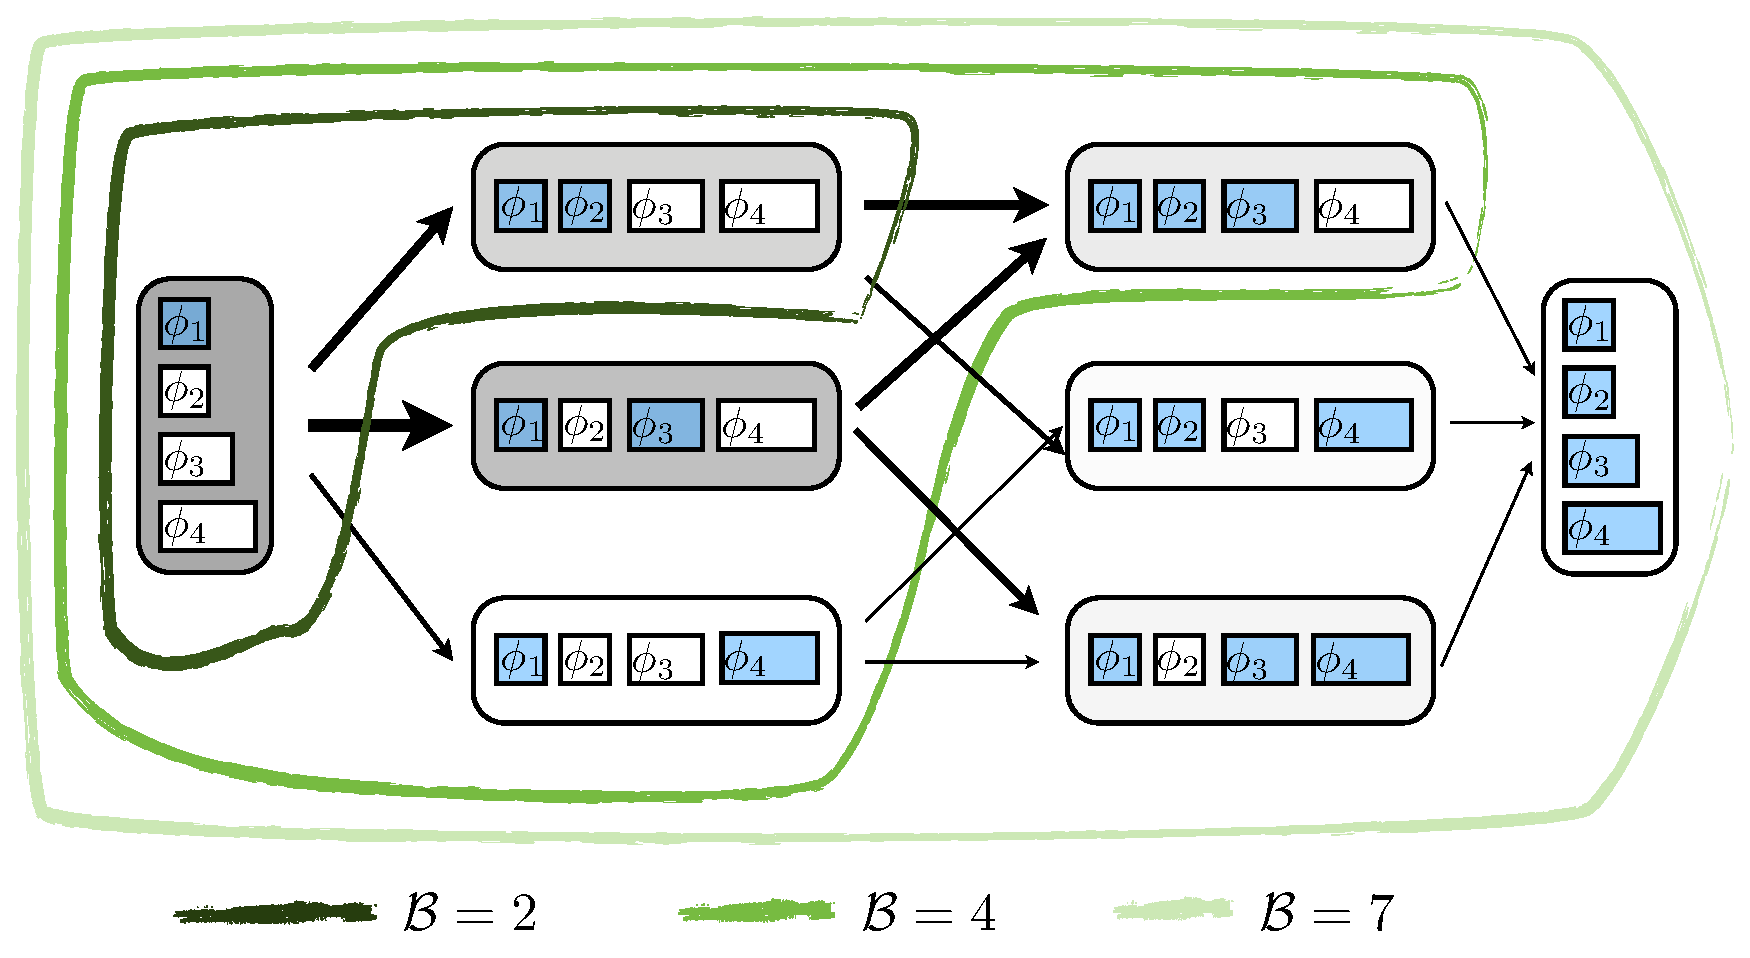
\includegraphics[width=.8\linewidth]{../../figures/mdp_masks.pdf}
\caption{
The action space $\mathcal{A}$ of the MDP is the the set of features $\mathcal{H}$, represented by the $\phi$ boxes.
The primary discretization of the state space can be visualized by the possible feature subsets (larger boxes); selected features are colored in the diagram.
The feature selection policy $\pi$ induces a distribution over feature subsets, for a dataset, which is represented by the shading of the larger boxes.
Not all states are reachable for a given budget $\mathcal{B}$.
In the figure, we show three ``budget cuts'' of the state space.
\label{fig:mdp_masks}
}
\end{figure}


As illustrated in \hyperref[fig:mdp_masks]{Figure~\ref*{fig:mdp_masks}}, the policy $\pi$ selects some feature subsets more frequently than others.
Instead of learning only one classifier $g$ that must be robust to all observed feature subsets, we can learn several classifiers, one for each of the most frequent subsets.
This is done by maintaining a distribution over encountered feature subsets during training.

We use hierarchical agglomerative clustering, growing clusters bottom-up from the observed masks.
In the case of training $K$ classifiers, we need to find $K$ clusters such that the masks are distributed as evenly as possible into the clusters.
The distance measure for the binary masks is the Hamming distance; standard K-Means clustering technique is not applicable to this distance measure.
Each one of $K$ classifiers is trained with the \textsc{Liblinear} implementation of logistic regression, with $L_2$ regularization parameter K-fold cross-validated at each iteration.
